% ########## Stammdaten ########## %

\newcommand{\Titel}{Vorlage zur Erstellung von Projektarbeiten an der Dualen-Hochschule-Gera-Eisenach}
\newcommand{\ProjektarbeitNummer}{2}
\newcommand{\Autor}{Max Mustermann}
\newcommand{\Matrikelnummer}{G000000PI}
\newcommand{\Campus}{Gera}
\newcommand{\Studienbereich}{Technik}
\newcommand{\Studiengang}{Komplexe Informatik}
\newcommand{\Kurs}{KIA89}
\newcommand{\Firma}{Musterfirma GmbH}
\newcommand{\BetreuerFirma}{Max Mustermann}
\newcommand{\BetreuerDHGE}{Moritz Mustermann}
\newcommand{\Abgabedatum}{02.05.2025}

% ########## Dokument Einstellungen ########## %

\documentclass[a4paper, 11pt]{article}

% ##########  Pakete ########## %

% ++++++++ Text +++++++++ %

\usepackage{acronym}
\usepackage[ngerman]{babel}
\usepackage[style=alphabetic, url=true, dateabbrev=false]{biblatex}
\addbibresource{bib.bib}

\usepackage{
  setspace,
  tocloft,
  csquotes,
  fancyhdr,
  enumitem,
  caption,
  amsmath,
  amssymb,
  amsthm,
  siunitx,
  soul,
  DHGEBiblatex
}
\usepackage[T1]{fontenc}
\usepackage[table]{xcolor}

% ++++++++  Grafiken +++++++++ %

\usepackage{wrapfig, graphicx, listings, geometry, tabularx, pdfpages, pdflscape}

% ++++++++ Fußnoten und Verlinkung +++++++++ %

\usepackage[hidelinks]{hyperref}

\hypersetup{
  pdftitle={Projektarbeit \ProjektarbeitNummer},
  pdfauthor={\Autor},
  pdfsubject={\Titel},
}

% ########## Seiten Einstellungen ########## %

\geometry{a4paper, left=3cm, right=2cm, top=2.5cm, bottom=2.5cm}
\setlength{\parindent}{0pt}
\setlength{\parskip}{6pt}
\onehalfspacing

% ########## Aufzählungen ########## %

\setlist[itemize,1]{leftmargin=10pt}

% ########## Bilder ########## %

% Beschriftung formatieren
\captionsetup{justification=raggedright,singlelinecheck=false}

% Rahmen Dicke
\setlength{\fboxrule}{1pt}
\setlength{\fboxsep}{0pt}

% ########## Text ########## %

\usepackage[scaled]{helvet}
\renewcommand{\familydefault}{\sfdefault}

% Nummern gleich formattiert wie Text
\sisetup{mode = text, detect-family = true, detect-weight = true}

% ########## Code Snippets ########## %

\lstdefinestyle{code}{
  columns=fullflexible,
  numbers=left,
  xleftmargin=30px,
  frame=single,
  framerule=1pt,
  framexleftmargin=25px,
  commentstyle=\color{gray},
  keywordstyle=\color{blue},
  numberstyle=\color{black},
  stringstyle=\color{gray},
  basicstyle=\ttfamily\footnotesize,
  captionpos=b,
  keepspaces=true,
  showstringspaces=false,
  escapechar=§
}
\lstset{style=code}

% ########## Kopf-/ & Fußzeile ########## %

% Textstyle
\pagestyle{fancy}
\renewcommand{\headrulewidth}{0pt}
\fancyhf{}
\fancyfoot[R]{\thepage}
\addtolength{\skip\footins}{3pc}

% Textstyle Inhaltsverzeichnis
\fancypagestyle{sxoli1}{
  \fancyhf{}
  \pagenumbering{Roman}
  \rfoot{\thepage}
  \renewcommand{\headrulewidth}{0pt}
  \renewcommand{\footrulewidth}{0pt}
	\fancypagestyle{plain}{
    \rfoot{\thepage}
	}
}

% ########## Verzeichnis Einstellungen ########## %

\renewcommand{\cftpartleader}{\cftdotfill{\cftdotsep}}
\renewcommand{\cftsecleader}{\cftdotfill{\cftdotsep}}
\renewcommand{\cftfigaftersnum}{:}
\renewcommand{\cfttabaftersnum}{:}
\renewcommand{\cftsecfont}{}
\renewcommand{\cftsecpagefont}{}
\setlength{\cftsecnumwidth}{50px}
\setlength{\cftsecindent}{0px}
\setlength{\cftsubsecnumwidth}{50px}
\setlength{\cftsubsecindent}{0px}
\setlength{\cftsubsubsecnumwidth}{50px}
\setlength{\cftsubsubsecindent}{0px}

% ########## Dokument Beginn ########## %
\begin{document}
% Keine Seitenzahlen auf Deckblatt und Sperrvermerk
\pagenumbering{gobble}

% ########## Deckblatt ########## %

\newcommand{\ProjektarbeitBoxen}{
  \ifcase\ProjektarbeitNummer 
  \or $\boxtimes$\hspace{1cm}$\square$\hspace{1cm}$\square$\hspace{1cm}$\square$ 
  \or $\square$\hspace{1cm}$\boxtimes$\hspace{1cm}$\square$\hspace{1cm}$\square$
  \or $\square$\hspace{1cm}$\square$\hspace{1cm}$\boxtimes$\hspace{1cm}$\square$
  \or $\square$\hspace{1cm}$\square$\hspace{1cm}$\square$\hspace{1cm}$\boxtimes$
  \fi
}

\begin{center}
  \textbf{\Titel}
  \vspace*{1cm}
\end{center}
\begin{center}
  \begin{tabular}{ r p{10cm} }
    Projektarbeit & {\LARGE\bf\hspace{0.15cm}I\hspace{1.225cm}II\hspace{1.05cm}III\hspace{1cm}IV}\\
    Nr. & {\LARGE\bf \ProjektarbeitBoxen}\\[1.5cm]
    & \Abgabedatum \\[-0.5cm]
    vorgelegt am: & \hrulefill \\[1cm]
    & \Autor \\[-0.5cm]
    von: & \hrulefill \\[1cm]
    & \Matrikelnummer \\[-0.5cm]
    Matrikelnr: & \hrulefill \\[1cm]
    & \Campus \\[-0.5cm]
    DHGE Campus: & \hrulefill \\[1cm]
    & \Studienbereich \\[-0.5cm]
    Studienbereich & \hrulefill \\[1cm]
    & \Studiengang \\[-0.5cm]
    Studiengang: & \hrulefill \\[1cm]
    & \Kurs \\[-0.5cm]
    Kurs: & \hrulefill \\[1cm]
    & \Firma \\[-0.5cm]
    Ausbildungsstätte: & \hrulefill \\[1cm]
    & \BetreuerFirma \\[-0.5cm]
    Betreuer: & \hrulefill \\[1cm]
    & \BetreuerDHGE \\[-0.5cm]
    & \hrulefill \\[1cm]
 \end{tabular}
\end{center}
\newpage

% ########## Sperrvermerk ########## %
\begin{center}
  \vspace*{5.5cm}
  {\LARGE\bf Sperrvermerk}
  \vspace*{1cm}
\end{center}

Die vorgelegte Projektarbeit mit dem Titel \enquote{\Titel} basiert auf internen, vertraulichen Daten und Informationen des Unternehmens \Firma.

Diese Projektarbeit darf nur vom Erst- und Zweitgutachter sowie berechtigten Mitgliedern des Prüfungsausschusses eingesehen werden.
Eine Vervielfältigung und Veröffentlichung der Projektarbeit ist auch auszugsweise nicht erlaubt.

Die Vervielfältigung und Veröffentlichung der Projektarbeit sowie die Einsichtnahme durch Dritte bedarf der ausdrücklichen
Zustimmung des Verfassers und des Unternehmens.
\newpage

% Römische Seitenzahl
\pagenumbering{Roman}

% ########## Inhaltsverzeichnis ########## %
\pagestyle{sxoli1}
\renewcommand{\contentsname}{Inhaltsverzeichnis}
\tableofcontents
\newpage

% ########## Abbildungsverzeichnis ########## %

\section*{Abbildungsverzeichnis}
\addcontentsline{toc}{section}{Abbildungsverzeichnis}

\renewcommand\listfigurename{}
\setlength{\cftfigindent}{0em}
\setlength{\cftfignumwidth}{6.5em}
\renewcommand{\cftfigpresnum}{Abbildung }
\listoffigures
\newpage

% ########## Tabellenverzeichnis ########## %

\section*{Tabellenverzeichnis}
\addcontentsline{toc}{section}{Tabellenverzeichnis}

\renewcommand\listtablename{}
\setlength{\cfttabindent}{0em}
\setlength{\cfttabnumwidth}{5.5em}
\renewcommand{\cfttabpresnum}{Tabelle }
\listoftables
\newpage

% ########## Abkürzungsverzeichnis ########## %
\phantomsection
\section*{Abkürzungsverzeichnis}
\addcontentsline{toc}{section}{Abkürzungsverzeichnis}
\begin{acronym}[**********]
  \acro{DHGE}{Duale Hochschule Gera Eisenach}
  \acro{VM}{Virtuelle Maschine}
  \acro{REST}{Representational State Transfer}
  \acro{RAG}{Retrieval-Augmented Generation}
 \end{acronym}
\newpage

% Falls Plural abweichend
\acrodefplural{VM}[VMs]{Virtuelle Maschinen}

% Letzte Seite mit römischer Seitenzahl speichern & Arabische Zahlen verwenden
\newcounter{savepage}
\setcounter{savepage}{\number\value{page}}
\pagenumbering{arabic}

% ########## Text ########## %

\section{Einleitung}

\subsection{Fließtext}
Lorem ipsum dolor sit amet, consetetur sadipscing elitr, sed diam nonumy eirmod tempor invidunt ut labore et dolore magna aliquyam erat, sed diam voluptua. At vero eos et accusam et justo duo dolores et ea rebum. Stet clita kasd gubergren, no sea takimata sanctus est Lorem ipsum dolor sit amet. Lorem ipsum dolor sit amet, consetetur sadipscing elitr, sed diam nonumy eirmod tempor invidunt ut labore et dolore magna aliquyam erat, sed diam voluptua. At vero eos et accusam et justo duo dolores et ea rebum. Stet clita kasd gubergren, no sea takimata sanctus est Lorem ipsum dolor sit amet. Lorem ipsum dolor sit amet, consetetur sadipscing elitr, sed diam nonumy eirmod tempor invidunt ut labore et dolore magna aliquyam erat, sed diam voluptua. At vero eos et accusam et justo duo dolores et ea rebum. Stet clita kasd gubergren, no sea takimata sanctus est Lorem ipsum dolor sit amet.
Duis autem vel eum iriure dolor in hendrerit in vulputate velit esse molestie consequat, vel illum dolore eu feugiat nulla facilisis at vero eros et accumsan et iusto odio dignissim qui blandit praesent luptatum zzril delenit augue duis dolore te feugait nulla facilisi. Lorem ipsum dolor sit amet, consectetuer adipiscing elit, sed diam nonummy nibh euismod tincidunt ut laoreet dolore magna aliquam erat volutpat.

\textit{kursiv text}    \textbf{fetter text}

\section{Kapitel}
\subsection{Unterkapitel}
\subsubsection{Unterunterkapitel}

\newpage

\section{Zitate}
Ein direktes Zitat \enquote{ist ein Zitat das sehr direkt ist.}\footnote{\cite{DIN.2008}}

dolore magna aliquyam erat, sed diam voluptua.\footnote{\cite{Fowler.2006} \cite{GitLab.2025}}

est Lorem ipsum dolor sit amet.\footnote{Ebd.}

\section{Auflistungen}

Die zentralen Merkmale von \acf{REST} sind:\footnote{Vgl. Ebd.}

\begin{itemize}
\item \textbf{Ressourcenidentifikation}\\
Jede Ressource in einem REST-System muss eindeutig identifizierbar sein, typischerweise über eine URI. Diese Identifikatoren sollten stabil und unabhängig vom Kontext auflösbar sein.

\item \textbf{Einheitliche Schnittstelle}\\
REST verwendet eine standardisierte Schnittstelle, die meist durch HTTP-Methoden wie GET, POST, PUT und DELETE realisiert wird. Diese Einheitlichkeit vereinfacht die Interaktion und entkoppelt Client und Server, was eine unabhängige Entwicklung ermöglicht.

\item \textbf{Selbstbeschreibende Nachrichten}\\
Jede Nachricht zwischen Client und Server muss alle notwendigen Informationen enthalten, um sie korrekt interpretieren und verarbeiten zu können. Dadurch wird vermieden, dass Clients auf externe Dokumentation oder Vorwissen angewiesen sind.

\item \textbf{Hypermedia als Steuerung der Anwendungslogik}\\
REST-konforme Antworten sollten Hyperlinks zu verwandten Ressourcen enthalten, sodass Clients die Anwendung dynamisch navigieren können. Diese Prinzipien ermöglichen eine flexible und entdeckbare Steuerung des Anwendungszustands.

\item \textbf{Zustandslose Kommunikation}\\
REST verlangt zustandslose Interaktionen zwischen Client und Server. Jede Anfrage muss alle relevanten Informationen enthalten, sodass der Server keine Sitzungsdaten speichern muss. Dies vereinfacht das Serverdesign und verbessert die Skalierbarkeit.
\end{itemize}

\newpage

\section{Formeln und mathematische Darstellung}

\begin{table}
\begin{tabular}{|l|l|}
  \hline
  \href{https://oeis.org/wiki/List_of_LaTeX_mathematical_symbols}{Mathematische Grundsymbole} & $- + \div \ast \times \cdot$\\
  \hline
  \href{https://oeis.org/wiki/List_of_LaTeX_mathematical_symbols}{Griechische Symbole} & $\alpha \pi \Delta \Theta \vartheta \mu \Lambda$\\
  \hline
  Relations Operatoren &  $< > = \nless \ngtr \parallel \leq \geq \ngeqslant \perp \subset \not\supset \nparallel \subseteq \approx \sim \neq \mid$\\
  \hline
  \href{https://oeis.org/wiki/List_of_LaTeX_mathematical_symbols}{Mathematische Notation} & $\mathbb{R} \mathbb{G} \mathbb{C} \in \notin \exists \overline{ab} f'(x)$\\
  \hline
  \href{https://oeis.org/wiki/List_of_LaTeX_mathematical_symbols}{Binär Operatoren} & $\neg \lor \land$\\
  \hline
  \href{http://namsu.de/Extra/befehle/Bruch.pdf}{Brüche} & $\frac{100}{(x \times y)^2}$\\
  \hline
  \href{https://www.namsu.de/Mathematik/1-6-2.html}{Wurzel} & $\sqrt[n]{\frac{100}{(x \times y)^2}}$\\
  \hline
  \href{https://de.overleaf.com/learn/latex/Integrals%2C_sums_and_limits}{Summen} & $\sum_{n=0}^{\infty}\frac{10}{n^2+1}$\\
  \hline
  \href{https://de.overleaf.com/learn/latex/Integrals%2C_sums_and_limits}{Integral} & $\int_sx^2*\frac{20}{dx}$\\
  \hline
  \href{https://de.overleaf.com/learn/latex/Integrals%2C_sums_and_limits}{Limes} & $lim_{x\to \infty} x$ eine Formel\\
  \hline
  \href{https://www.overleaf.com/learn/latex/Matrices}{Matrizen} &
$\begin{pmatrix}
  1 & 1 & 1\\
  0 & 0 & 1\\
  1 & 0 & 1
\end{pmatrix}$
$\begin{bmatrix}
  1 & 1 & 1\\
  0 & 0 & 1\\
  1 & 0 & 1
\end{bmatrix}$\\
\hline
\href{https://www.overleaf.com/latex/examples/cases/nndqpbymnchn}{Fälle} & 
$|x|=
\begin{cases}
x & \text{ für } x < 0\\
x & \text{ für } x > 100\\
0 & \text{ für } x = 0
\end{cases}$\\
\hline
\end{tabular}
\caption{Tabelle mit Mathe}
\end{table}

\subsection{Mathe in mehreren Zeilen}

\begin{align}
  f(x)&=\sqrt[3]{\frac{x}{z^2}} &f(x)&=x^2+bx+q\\
  h(x)&=\frac{n^2}{\sqrt{x-2}} &h(x)&=\sqrt{n}\ast n+f(x)^2\notag
\end{align}

\subsection{Große Zahlen und Einheiten darstellen}

\href{https://texdoc.org/serve/siunitx/0}{Bedienungsanleitung}

\num{100000}

\num{200000000.000000}

\num{300000000000000}

\qty{40}{\percent}

\qty{5}{\texteuro}

\qty{6}{\textdollar}
\newpage

\section{Abkürzungen}

\begin{table}[h]
  \centering
\begin{tabular}{|l|l|}
\hline
\multicolumn{2}{|c|}{\href{https://www.namsu.de/Extra/pakete/Acronym.html}{Bedienungsanleitung (acronym)}}\\
\hline
Normal & \ac{DHGE}\\
\hline
Abkürzung & \acs{DHGE}\\
\hline
Langform & \acl{DHGE}\\
\hline
Langform + Abkürzung & \acf{DHGE}\\
\hline
Keine Langform + Plural & \acp{DHGE}\\
\hline
Kurzform + Plural & \acsp{DHGE}\\
\hline
Langform + Plural & \acfp{DHGE}\\
\hline
Langform + Abkürzung + Plural & \aclp{DHGE}\\
\hline
Abweichender Plural & \acp{VM}\\
\hline
\end{tabular}
\caption{Abkürzungen im Text nutzen}
\end{table}

\section{Grafiken}

\subsection{Bilder}

\par\medskip
\begin{figure}[!ht]
    \centering
    \frame{\includegraphics[width=\textwidth]{example-image-a}}
    \caption[Ein Bild]{Ein Bild\protect\footnotemark}
    \label{fig:ExampleImage}
\end{figure}

\footnotetext{\href{https://texdoc.org/serve/graphicx.pdf/0}{Bedienungsanleitung (Graphicx)}}

\subsection{Bilder neben Text}

\par\medskip
\begin{wrapfigure}[12]{r}[0pt]{5cm}
    \centering
    \frame{\includegraphics[width=0.3\textwidth]{example-grid-100x100pt}}
    \caption[Eingerücktes Bild]{Eingerücktes Bild\protect\footnotemark}
    \label{fig:ExampleFloatImage}
\end{wrapfigure}
\footnotetext{\href{https://ctan.ebinger.cc/tex-archive/macros/latex/contrib/wrapfig/wrapfig-doc.pdf}{Bedienungsanleitung (wrapfig)}}
Lorem ipsum dolor sit amet, consetetur sadipscing elitr, sed diam nonumy eirmod tempor invidunt ut labore et dolore magna aliquyam erat, sed diam voluptua. At vero eos et accusam et justo duo dolores et ea rebum. Stet clita kasd gubergren, no sea takimata sanctus est Lorem ipsum dolor sit amet. Lorem ipsum dolor sit amet, consetetur sadipscing elitr, sed diam nonumy eirmod tempor invidunt ut labore et dolore magna aliquyam erat, sed diam voluptua. At vero eos et accusam et justo duo dolores et ea rebum. Stet clita kasd gubergren, no sea takimata sanctus est Lorem ipsum dolor sit amet. Lorem ipsum dolor sit amet, consetetur sadipscing elitr, sed diam nonumy eirmod tempor invidunt ut labore et dolore magna aliquyam erat, sed diam voluptua. At vero eos et accusam et justo duo dolores et ea rebum. Stet clita kasd gubergren, no sea takimata sanctus est Lorem ipsum dolor sit amet.
Duis autem vel eum iriure dolor in hendrerit in vulputate velit esse molestie consequat, vel illum dolore eu feugiat nulla facilisis at vero eros et accumsan et iusto odio dignissim qui blandit praesent luptatum zzril delenit augue duis dolore te feugait nulla facilisi. Lorem ipsum dolor sit amet, consectetuer adipiscing elit, sed diam nonummy nibh euismod tincidunt ut laoreet dolore magna aliquam erat volutpat.

\clearpage

\subsection{Weitere Grafikbeispiele mit \href{https://tikz.dev/}{Tikz}}

\begin{figure}[!ht]
  \centering
    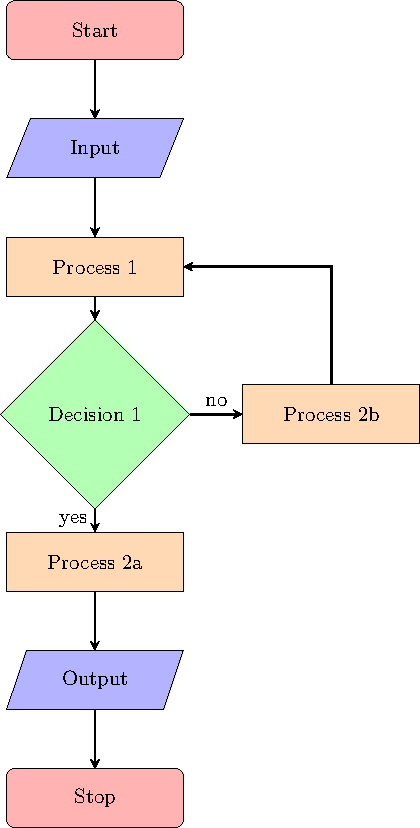
\includegraphics{Grafiken/Flussdiagramm.pdf}
  \caption{Flussdiagramm nach DIN 66001}
  \label{fig:ExampleFlowchart}
\end{figure}

\clearpage

\begin{figure}[!ht]
  \centering
    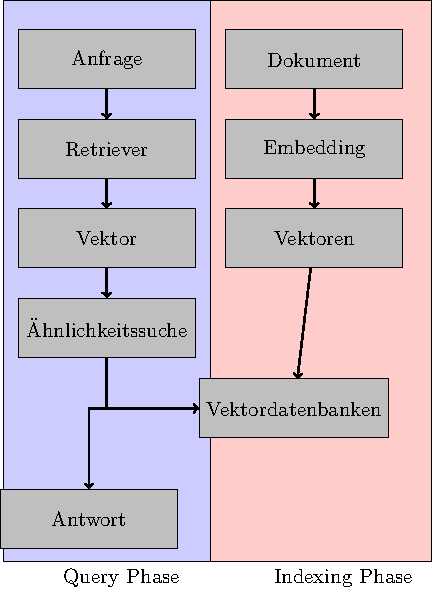
\includegraphics{Grafiken/RAG.pdf}
  \caption[Vereinfachte Darstellung der Funktionsweise eines \acs{RAG}]{Vereinfachte Darstellung der Funktionsweise eines \acs{RAG}\protect\footnotemark}
  \label{fig:vektordatenbanken}
\end{figure}
\footnotetext{Darstellung nach \cite{LangChain.2025-Docs-Vektordatenbanken} nachgebildet}

\clearpage

\begin{figure}[!ht]
  \centering
    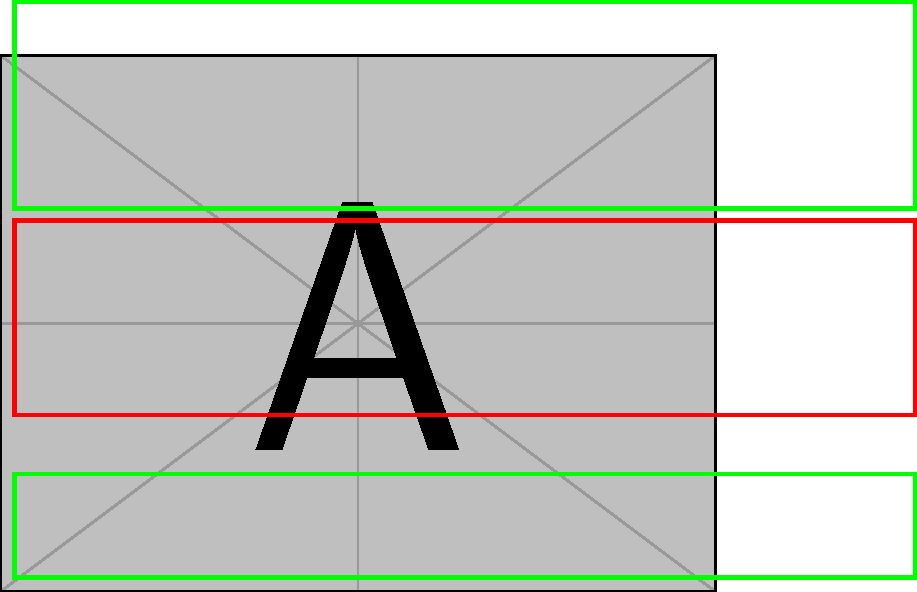
\includegraphics[width=0.8\textwidth]{Grafiken/Markiert.pdf}
  \caption{Rahmen in Bilder einfügen}
  \label{fig:rahmenInBilder}
\end{figure}

\clearpage

\subsection{Code einfügen}

\begin{figure}[!ht]
\begin{lstlisting}[language=Python]
import random as randintint 
number = randint(1, 10)
def main(argv):
    return 0
\end{lstlisting}
\caption[Titel]{Titel\protect\footnotemark}
\label{fig:ExampleCode}
\end{figure}
\footnotetext{\href{https://texdoc.org/serve/listings.pdf/0}{Bedienungsanleitung (listings)}}

\sethlcolor{yellow}
\begin{figure}[!ht]
\begin{lstlisting}[language=c]
int tls1_process_heartbeat(SSL *s) {
  unsigned char *p = &s->s3->rrec.data[0], *pl;
  unsigned short hbtype;
  unsigned int payload;
  unsigned int padding = 16;

  §\hl{/* Read type and payload length first */}§
  §\hl{hbtype = *p++;}§
  §\hl{n2s(p, payload);}§
  §\hl{pl = p;}§
\end{lstlisting}
\caption[Betroffener Code aus der OpenSSL Bibliothek]{Betroffener Code aus der OpenSSL Bibliothek (in \hl{gelb} fehlerhafter Code)\protect\footnotemark}
\label{fig:ExampleCode2}
\end{figure}
\footnotetext{\href{https://texdoc.org/serve/listings.pdf/0}{Bedienungsanleitung (listings)}}
\clearpage

\subsection{Ordnerstrukturen}

\begin{figure}[!ht]
  \centering
    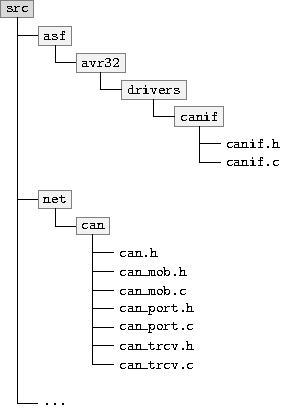
\includegraphics[width=0.5\textwidth]{Grafiken/Ordnerstruktur.pdf}
  \caption{Ordnerstrukturen mit Tikz}
  \label{fig:Ordnerstrukturen}
\end{figure}
\clearpage

% ########## Literaturverzeichnis ########## %

% Römische Seitenzahlen fortsetzen
\pagenumbering{Roman}
\setcounter{page}{\value{savepage}}

\phantomsection
\section*{Literaturverzeichnis}
\addcontentsline{toc}{section}{Literaturverzeichnis}
\renewcommand\refname{}
\printbibliography
\newpage

% ########## Anlagen ########## %
\phantomsection
\section*{Anlagenverzeichnis}
\addcontentsline{toc}{section}{Anlagenverzeichnis}
\captionsetup[figure]{list=no}
\setcounter{figure}{0}
\renewcommand{\figurename}{Anhang}
\renewcommand{\thefigure}{\arabic{figure}}

% Anlagenverzeichnis (muss manuell geführt werden)
\renewcommand\tabularxcolumn[1]{b{#1}}
\renewcommand*{\arraystretch}{1.5}
\begin{tabularx}{\textwidth}{Xr}
\multicolumn{2}{c}{}\\
Anhang 1: \nameref{Anhang:1} \dotfill&\pageref{Anhang:1}\\
Anhang 2: \nameref{Anhang:2} \dotfill&\pageref{Anhang:2}\\
Anhang 3: \nameref{Anhang:3} \dotfill&\pageref{Anhang:3}\\
\end{tabularx}
\newpage

% ########## Anlage 1 ########## %

\begin{figure}[!ht]
  \caption[Titel im Anlagenverzeichnis Anlage 1]{Titel Anlage 1}
  \label{Anhang:1}
  \centering
  \frame{\includegraphics[angle=-90, width=\textwidth]{example-image-a}}
\end{figure}
\newpage

% ########## Anlage 2 ########## %

\begin{landscape}
  \begin{figure}[!ht]
    \caption[Titel im Anlagenverzeichnis Anlage 2]{Titel Anlage 2}
    \label{Anhang:2}
    \centering
    \frame{\includegraphics[width=1.2\textwidth]{example-image-a}}
  \end{figure}
  \end{landscape}
  \newpage

% ########## Anlage 3 ########## %

\begin{figure}[!ht]
  \caption[Titel im Anlagenverzeichnis Anlage 3]{Titel Anlage 3}
  \label{Anhang:3}
  \centering
  \frame{\includegraphics[angle=-90, width=\textwidth]{example-image-a}}
\end{figure}
\newpage

% ########## Eigenständigkeitserklärung ########## %

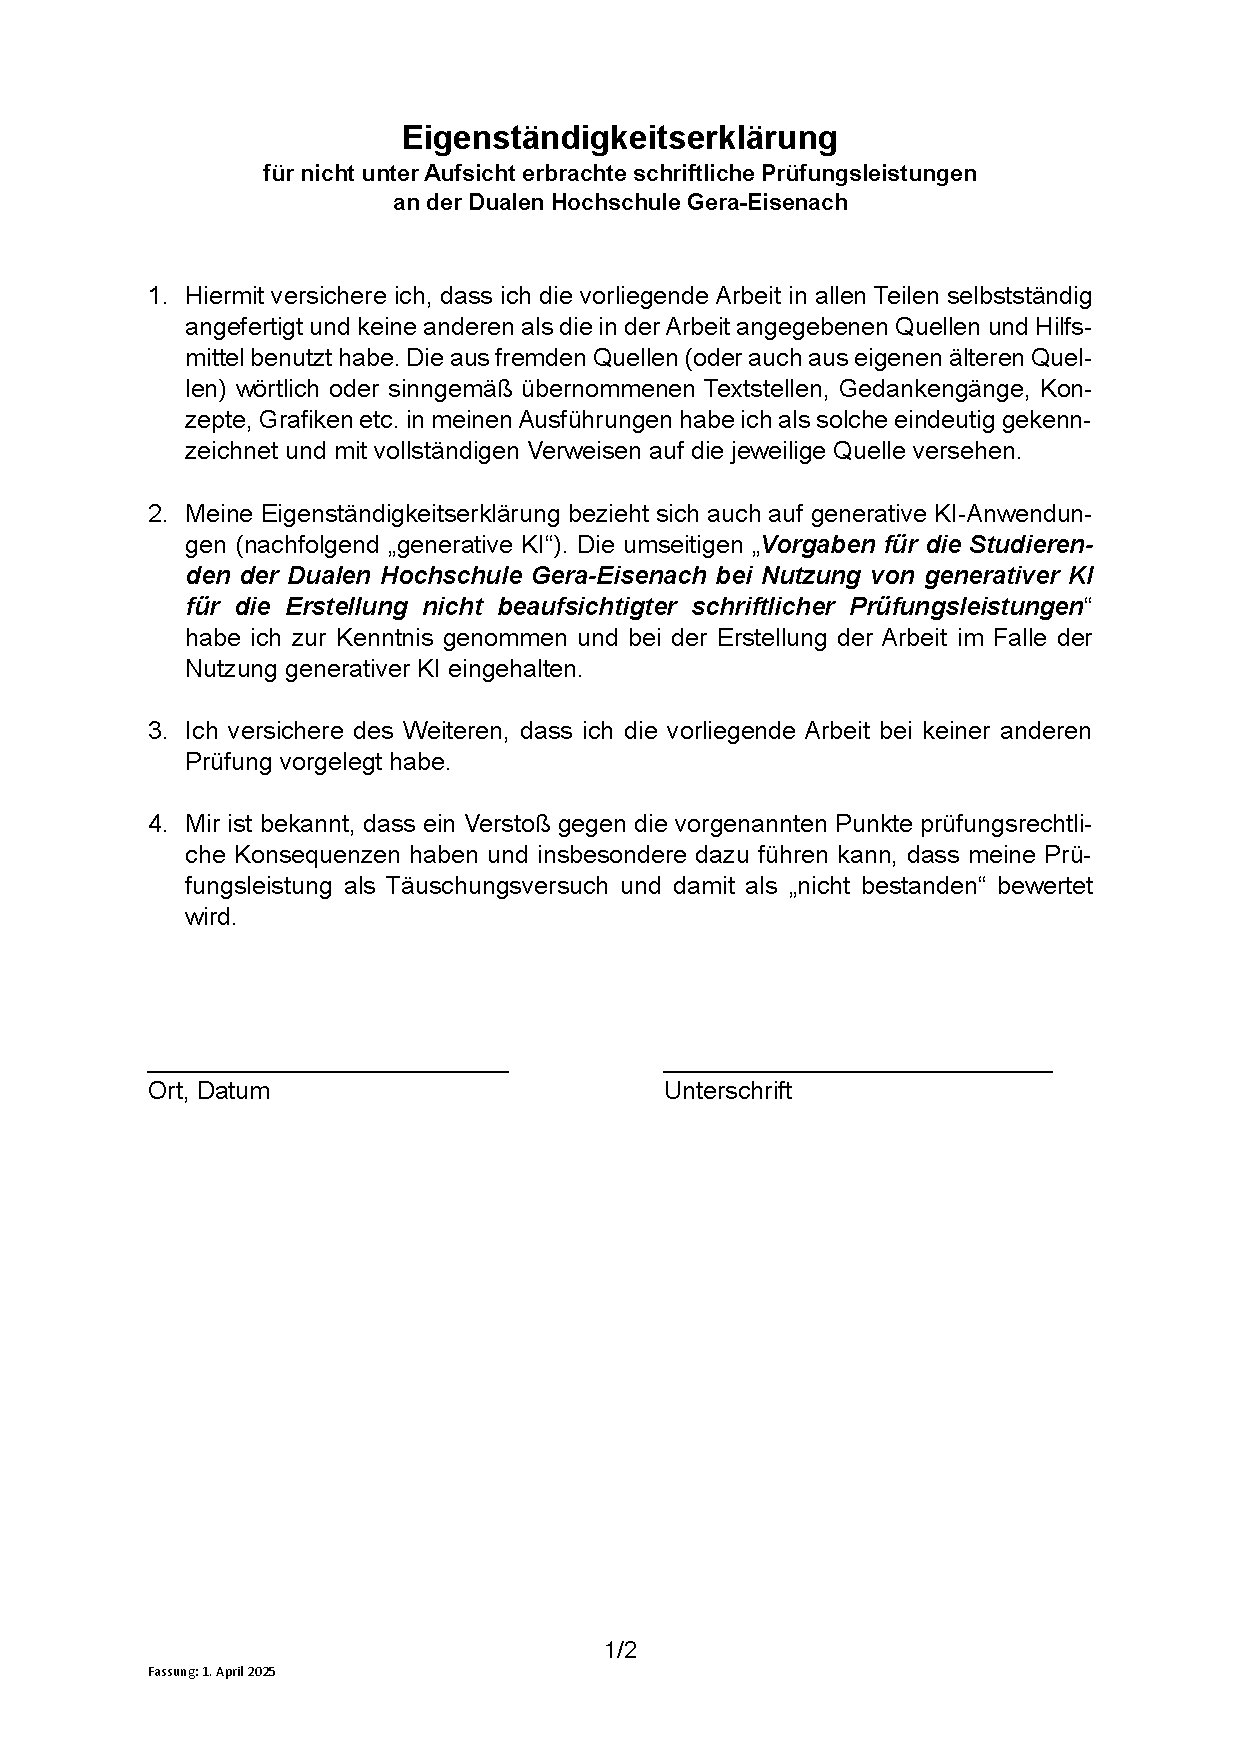
\includepdf[pages=-]{Eigenständigkeitserklärung.pdf}

\end{document}